
%(BEGIN_QUESTION)
% Copyright 2009, Tony R. Kuphaldt, released under the Creative Commons Attribution License (v 1.0)
% This means you may do almost anything with this work of mine, so long as you give me proper credit

Determine the voltages registered by a voltmeter between the following points in this circuit.  Be sure to note whether the voltmeter's indication will be a positive value or a negative value in each case:

$$\includegraphics[width=15.5cm]{i02520x01.eps}$$

$V_A = \hbox{\underbar{ \hskip 20pt}}$ (red lead on {\bf A}, black lead on ground)

\vskip 5pt

$V_B = \hbox{\underbar{ \hskip 20pt}}$ (red lead on {\bf B}, black lead on ground)

\vskip 5pt

$V_C = \hbox{\underbar{ \hskip 20pt}}$ (red lead on {\bf C}, black lead on ground)

\vskip 5pt

$V_D = \hbox{\underbar{ \hskip 20pt}}$ (red lead on {\bf D}, black lead on ground)

\vskip 20pt

$V_{AC} = \hbox{\underbar{ \hskip 20pt}}$ (red lead on {\bf A}, black lead on {\bf C})

\vskip 5pt

$V_{DB} = \hbox{\underbar{ \hskip 20pt}}$ (red lead on {\bf D}, black lead on {\bf B})

\vskip 5pt

$V_{BA} = \hbox{\underbar{ \hskip 20pt}}$ (red lead on {\bf B}, black lead on {\bf A})

\vskip 5pt

$V_{BC} = \hbox{\underbar{ \hskip 20pt}}$ (red lead on {\bf B}, black lead on {\bf C})

\vskip 5pt

$V_{CD} = \hbox{\underbar{ \hskip 20pt}}$ (red lead on {\bf C}, black lead on {\bf D})

\underbar{file i02520}
%(END_QUESTION)





%(BEGIN_ANSWER)

$V_A = \hbox{\underbar{ +30 volts}}$ (red lead on {\bf A}, black lead on ground)

\vskip 5pt

$V_B = \hbox{\underbar{ +3 volts}}$ (red lead on {\bf B}, black lead on ground)

\vskip 5pt

$V_C = \hbox{\underbar{ +9 volts}}$ (red lead on {\bf C}, black lead on ground)

\vskip 5pt

$V_D = \hbox{\underbar{ -15 volts}}$ (red lead on {\bf D}, black lead on ground)

\vskip 20pt

\goodbreak

$V_{AC} = \hbox{\underbar{ +21 volts}}$ (red lead on {\bf A}, black lead on {\bf C})

\vskip 5pt

$V_{DB} = \hbox{\underbar{ -18 volts}}$ (red lead on {\bf D}, black lead on {\bf B})

\vskip 5pt

$V_{BA} = \hbox{\underbar{ -27 volts}}$ (red lead on {\bf B}, black lead on {\bf A})

\vskip 5pt

$V_{BC} = \hbox{\underbar{ -6 volts}}$ (red lead on {\bf B}, black lead on {\bf C})

\vskip 5pt

$V_{CD} = \hbox{\underbar{ +24 volts}}$ (red lead on {\bf C}, black lead on {\bf D})


%(END_ANSWER)





%(BEGIN_NOTES)


%INDEX% Electronics review: Kirchhoff's Voltage Law (KVL)

%(END_NOTES)


